\documentclass[conference, 11pt]{IEEEtran}
\usepackage{graphicx, indentfirst}
\usepackage{url}
\usepackage{hyperref}
\usepackage{siunitx}
\usepackage{amsmath}



\title{A Comparative Analysis of SAC, TD3, and DWA for Mapless Goal-Directed Navigation in Unknown Environments.}
\author{
\IEEEauthorblockA{CSCI 5551: Introduction to Intelligent Robotic Systems}
    \IEEEauthorblockN{Ketan Inampudi (inamp005@umn.edu), Alec Olson (ols00160@umn.edu)} \\
}
\date{November 20, 2026}

\begin{document}

\maketitle

\section{Abstract}
Autonomous mobile robots are often required to navigate unknown environments to reach prespecified goals safely. 
In many real-world settings, however, a prior map of the environment may not be available, requiring the robot to navigate the unknown environment using only local sensor observations and relative goal information.
Mapless navigation methods allow a mobile robot to make navigation decisions without relying on a complete representation of the environment. 
This project will investigate whether Deep Reinforcement Learning (DRL) methodologies can perform mapless navigation to reach a goal using range measurements collected from a LiDAR sensor, relative goal distance, and relative goal bearing. 
Two DRL algorithms, Soft Actor-Critic (SAC) and Twin Delayed Deep Deterministic Policy Gradient (TD3), will be compared against the Dynamic Window Approach (DWA) under common environmental constraints. 
Training will be completed inside a simulated physics environment with randomized unknown environments being generated. Evaluation of DRL algorithms alongside DWA will be done in both simulated environments and previously unseen real-world environments with the use of a TurtleBot3 mobile robot. 
Performance will be compared using measures such as navigation success, collision rate, path efficiency, and time to goal.

\section{Problem Description}
Autonomous mobile robots are widespread in society today and have applications in many domains, including navigating warehouses \cite{keith2024reviewautonomousmobilerobots}, healthcare environments \cite{electronics12234791}, agriculture, manufacturing, and transportation \cite{electronics13030542}.
Many of these applications of autonomous mobile robots allow for the robot to be given a clear definition of the environment it is tasked with navigating; for example, warehouses and hospitals are clearly defined environments where the locations of stations and equipment are generally well known.
In these applications, a detailed map of the environment may be available, allowing the robot to localize itself and globally plan a route to its destination. 
In other applications, a prior map is not available, which requires the robot to navigate the environment using another technique, such as, simultaneous localization and mapping (SLAM), where the robot can estimate its position while constructing a representation of the environment \cite{Durrant_Bailey} \cite{Loganathan}.
The standard approach of using SLAM along with a path planning algorithm and control system performs well in static environments.
However, such static environments are not always guaranteed, and with the introduction of dynamically changing environments or stricter time restrictions, the standard approach becomes increasingly less feasible. 
With dynamic environments, sustaining a map of the environment becomes impractical with constantly changing landmarks and obstacles leading to a high computational cost as the environment changes \cite{past-present-future-slam}.
Additionally, there may be environments in which the robot needs to be operational immediately without time to learn the environment through exploration. 
For such cases, mapless goal-directed navigation methods can be employed which would allow the robot to only use local sensor information along with relative goal information \cite{Dobrevski_Skočaj_2021}.
This project aims to explore such kinds of navigation methods in mobile robots that may be deployable in previously unseen dynamic environments \cite{Tai_Lei}.
\par
The first algorithm that will be evaluated in unknown environments will be the Dynamic Window Approach, which will work as a baseline against which to evaluate the remaining two DRL algorithms.
DWA is a local reactive method that allows for collision avoidance and local motion planning \cite{Fox_Burgand}.
DWA approaches the problem of both local motion planning and collision avoidance by first directly searching the space of velocities and secondly choosing the velocities that maximize an objective function. 
This is done by accounting for the actual motion dynamics of the robot, considering what velocities are attainable within the dynamic window, and rejecting unsafe velocities in order to prune the search space.
Then, velocities are chosen via the objective function which considers progress towards the goal, clearance of nearby obstacles, and velocity of the robot. 
Choosing velocities by maximizing this objective function allows the DWA to perform mapless goal-directed navigation in unseen environments without needing a learning algorithm or any previous training.
\par
The two DRL algorithms chosen for this project are Soft Actor-Critic (SAC) and Twin Delayed Deep Deterministic Policy Gradient (TD3).
These DRL algorithms were chosen because they are both designed for continuous control problems which makes them suitable for robot navigation problems where state, observation, and especially action spaces are all continuous \cite{deJesus_SAC_Nav} \cite{Cimurs_TD3_Nav}.
SAC is an off-policy actor-critic algorithm that is capable of learning both a policy and value function \cite{Haarnoja_SAC}.
SAC also maximizes the expected reward while also encouraging policy entropy.
As a result, SAC is able to encourage exploration while helping reduce premature convergence due to poor decisions.
TD3 is also an off-policy actor-critic algorithm; however, TD3 was designed to reduce value-estimation errors that would otherwise destabilize similar deterministic continuous control algorithms \cite{Fujimoto_TD3}.
TD3 addresses this by using two critic networks, delayed policy updates, and target-policy smoothing.
Both DRL algorithms have previously been used in continuous robotic control problems, and DRL has been applied to mapless mobile robot navigation using local range sensing and relative target information \cite{Tai_Lei} \cite{8202312}.
Comparing SAC and TD3 under the same navigation tasks will allow us to evaluate how differences in their policy-learning and value-estimation strategies affect navigation reliability, efficiency, and generalization \cite{Dobrevski_Skočaj_2021} \cite{Tai_Lei}.

The experiments we complete will compare SAC, TD3, and the DWA under a common mapless goal-directed navigation framework.
Each method will receive comparable local range measurements, the distance and bearing to the goal, and the robot's current motion information.
Using the information provided, each method will generate a translational and rotational velocity command for a differential-drive mobile robot. 
SAC and TD3 will be trained in a physics-based simulation which will randomly generate starting positions, goal locations, static obstacles, and some dynamic obstacles. 
DWA will operate without training as the classical baseline, since it is not a learned algorithm \cite{Fox_Burgand}.
After training, the learned policies from SAC and TD3 will be frozen and evaluated together with DWA in previously unseen environments to ensure the performance reflects generalization rather than memorization.
The methods will be compared using metrics such as goal-reaching success rate, collision rate, path length, travel time, path efficiency, and obstacle clearance.
Once the simulated policies are reliably performing in the simulated environments, the same navigation approaches will be tested on a TurtleBot3, implemented with ROS \cite{ros-open-source-operating-system}, in controlled indoor environments to evaluate simulation to real transfer \cite{Tai_Lei} \cite{Yan_2D}.

\section{Methods}
This section describes the simulated environment, the learning problem given to each agent, and the configuration of the two DRL algorithms for this first training round.

\subsection{Simulation Environment Setup}

A simulated environment was created to train a robot and begin to investigate the differences between SAC and TD3 before moving to the real TurtleBot3. The environment uses the MuJoCo physics engine \cite{Todorov_MuJoCo} with a model of the TurtleBot3 Burger, and the agents were trained with the Stable-Baselines3 implementations of SAC and TD3 \cite{Raffin_SB3}. The environment was setup with the following parameters:

    \begin{itemize}
        \item \textbf{Room}: $6 \mathrm{m}$ x $6 \mathrm{m}$ with walls on all sides.
    
        \item \textbf{LiDAR}: $72$ beams at \ang{5} intervals, therefore covering all \ang{360}; maximum range of $3.5 \mathrm{m}$, which is the maximum range of the LDS-01 sensor on the TurtleBot3 Burger.

        \item \textbf{Control}: A new velocity command is issued every $0.2 \mathrm{s}$ ($5 \mathrm{Hz}$)
    
        \item \textbf{Start and Goal Positions}: Selected randomly from a uniform distribution within $2.5 \mathrm{m}$ of the center of the room. A heading angle $\theta$ is also defined for the starting position and is the direction the robot is initially facing.
    
        \item \textbf{Goal}: Success is defined as the robot reaching within $0.2 \mathrm{m}$ of the goal location.

        \item \textbf{Episode Termination}: An episode ends when one of the following happens:
            \begin{enumerate}
                \item The robot reaches the goal location.
    
                \item The robot collides with an obstacle or a wall.
    
                \item The robot reaches $600$ control steps, which is $120 \mathrm{s}$, and this causes the program to timeout.
            \end{enumerate}
    
        \item \textbf{Difficulty Levels}: Four difficulty levels are defined:
            \begin{enumerate}
                \item Empty: No obstacles in the environment.
                \item Sparse Static: One or two static obstacles in the environment.
                \item Dense Static: Between three and six (inclusive) static obstacles in the environment.
                \item Static and Moving: Between two and six (inclusive) static obstacles in the environment with one or two moving obstacles.
            \end{enumerate}
            These obstacles are also placed at random in the room. During training, $10\%$ of the episodes had a difficulty level of Empty, $10\%$ were Sparse Static, $15\%$ were Dense Static, and $65\%$ were Static and Moving.
    
        \item \textbf{Obstacles}: Circular objects with a radius between $0.15$ and $0.28 \mathrm{m}$. Moving obstacles oscillate in a sinusoidal pattern with an amplitude of $0.25 \mathrm{m}$ and a period of $12 \mathrm{s}$, which means their peak speed is approximately $0.13 \mathrm{m/s}$. Obstacles are placed so that the space swept by any two of them is separated by at least $0.35 \mathrm{m}$. This leaves a gap wide enough for the robot to pass through and also makes sure that no obstacle interferes with the start or goal location.
    \end{itemize}

\subsection{Observation and Action Spaces}
At each control step, the agent receives a $77$-dimensional observation vector. It is broken down into the following components:
    \begin{itemize}
        \item $72$ of these values are the LiDAR data for each beam. The distance measured is then divided by $3.5 \mathrm{m}$, which means this data lies in the range $[0, 1]$.

        \item The distance from the robot's current location to the goal location, divided by the distance between two corners of the room so that the value lies in $[0, 1]$. The room is $6 \mathrm{m}$ x $6 \mathrm{m}$, so this diagonal distance is $\sqrt{6^2 + 6^2} = \sqrt{72} \approx 8.49 \mathrm{m}$.

        \item The sine and cosine of the angle to the goal location, relative to the robot's heading. The domain of these values is already $[-1, 1]$, so no adjustment is needed.

        \item The robot's linear velocity $v$ and angular velocity $\omega$, scaled to fall in the range $[-1, 1]$ by dividing by the maximum possible values for the TurtleBot3: $0.22 \mathrm{m/s}$ for $v$ and $2.84 \mathrm{rad/s}$ for $\omega$.
    \end{itemize}

The robot has neither a map nor knowledge of the positions or velocities of the obstacles.

Each action is a $2$-dimensional vector that stores a linear velocity $v$ and an angular velocity $\omega$ which are used to drive the robot.

\subsection{Reward Function}
The reward function used combines progress toward the goal, time penalty, obstacle-proximity penalty, and terminal reward.
The same reward function is currently used for both the SAC and TD3 agents so that differences in performance can be tracked to differences in the algorithms rather than differences in task objectives. 
The reward at each step of the training is defined by the following equation:
    \begin{equation}
        r_t = 5(d_{t-1} - d_t) - 0.01 + r_{\mathrm{prox}} + r_{\mathrm{term}}
    \end{equation}

The parameters for the equation are:
    \begin{itemize}
        \item $t$: The current timestep.

        \item $d_t$: The distance in meters from the robot to the goal location at timestep $t$.

        \item $l_t$: The current smallest LiDAR measurement.

        \item $r_{\mathrm{prox}}$: Proximity from the robot to the nearest wall or obstacle, defined as:
            \begin{equation}
                max\Big(0, \frac{0.30-l_t}{0.30}\Big)
            \end{equation}

        \item $r_{\mathrm{term}}$: Terminal reward, $+10$ if the robot reaches the goal, $-10$ if it collides with a wall or obstacle, and $0$ else wise.
    \end{itemize}

For $r_{term}$, success is measured as the robot reaching within $0.20 \mathrm{m}$ of the goal without any collisions.
Contact with an obstacle or wall, leaving the boundaries, or excessive tile are all counted as collisions or failure. 
A training episode terminates upon either success or collision, and if a training episode exceeds 600 steps, the episode is terminated with no reward being given. 

The coefficients chosen are initial heuristic settings only intended to provide a starting point to gather useful feedback throughout training.
Further refinements to the reward function, and the coefficients used, will need to be done. 
The progress coefficient of 5 rewards the robot for making forward progress, even if the progress is relatively small. For example, if the robot moves $0.02 \mathrm{m}$ closer to the goal, the reward would be $0.10$. 
The reward for small increments towards the goal is meant to offset the time penalty of $-0.01$ that is encouraged when the robot is inactive and adds to the penalty of the robot making unnecessary movements. 

The proximity term introduces a gradual penalty when the robot travels too close to an obstacle or wall.
The penalty is incurred when a LiDAR measurement is less than $0.30 \mathrm{m}$.
That is, if the robot detects anything less than $0.30 \mathrm{m}$ from the origin of the LiDAR reading, it incurs a penalty. 
The $0.30 \mathrm{m}$ radius is a local caution region and not meant to represent any physically validated stopping distance. 

Finally, the terminal values of $+10$ and $-10$, for success and collision respectively, make those outcomes more impactful than any other movement reward. 
Thus, the agent learns to prioritize both reaching the goal and avoiding collisions. 
These choices allow for an initial balance between progress, speed, and clearance, but their effectiveness still needs to be revised based on the results of training and evaluation discussed in Section \ref{initial-results}. 

The current reward function has several consequences that impact the behavior being learned.
Since progress is measured using a straight line goal distance, any necessary obstacle avoidance will result in a negative reward (since the robot initially moves farther away from the goal). 
The agent must then learn that a temporary loss of progress can lead to better future outcomes. 
Additionally, the progress reward is accumulated by total net reduction of distance to goal rather than total distance traveled. 
So any additional travel is discouraged with the time penalty and potentially with the proximity penalty. 
There is no penalty for reversing, sharp turns, or changing actions abruptly.
As a result, the reward encourages navigation efficiency but does not require smooth, or energy efficient, movement. 

\subsection{Soft Actor-Critic}

Soft Actor-Critic is an off-policy actor-critic algorithm for continuous control. Its actor represents a probability distribution over actions, while its critic estimates the value of taking an action from a given observation. 
Experience is stored in a replay buffer and reused during learning. 
SAC optimizes both expected return and policy entropy, encouraging exploration while learning actions that improve task performance. 

In the SAC implementation used in this project, the stochastic actor is combined with the two critics and the smaller critic estimate is used when constructing learning targets.
The entropy coefficient is set to target $-2$ but is adjusted automatically to regulate policy randomness. 
The actor and critics are updated during each training iteration and the entropy regularization affects the agents learning objective bus is not captured as part of the results. 
During evaluation, deterministic action selection is used to measure the learned policy without stochastic action sampling. \cite{haarnojaSAC_Applications}

\subsection{Twin Delayed Deep Deterministic Policy Gradient}
Twin Delayed Deep Deterministic Policy Gradient is also a off-policy actor-critic algorithm that extends DDPG \cite{continuous-control-deep-rl}.
Its actor produces a deterministic action, while exploration is introduced separately during data collection. 
TD3 addresses value overestimation using two critics and the smaller target actions when construction critic targets.
These mechanisms are intended to reduce the effect of inaccurate value estimations on policy learning. 

TD3 uses a Gaussian exploration noise in the internally normalized action space. 
The actor and target networks are updated once every two critic-training iterations. 
Target-policy smoothing uses a noise standard deviation of $0.2$, clipped to $\pm 0.5$ in normalized coordinates; this is separate from the exploration noise applied during environment interaction.
The main distinction in comparison is therefore how exploration in incorporated: SAC learns a stochastic policy with entropy regularization, whereas TD3 trains a deterministic policy using externally added noise. 
Both are evaluated deterministically, and neither mechanism alone establishes which algorithm performs better on the navigation task. 

\section{Initial Results} \label{initial-results}
Each training round ran for $350,000$ steps, and the robot was given $600$ steps to reach the goal for each episode. As described earlier, if the robot could not reach the goal within this time, the episode was deemed a failure. Therefore, the minimum number of full episodes that the robot could train for was $\frac{350,000}{600} = 583$. However, the robot was able to perform many more episodes because it was generally able to reach the goal well under budget. For this first part of training, we ran three seed rounds each for SAC and TD3.

Figures \ref{fig:success_rate_sac_seed0}, \ref{fig:success_rate_td3_seed0}, \ref{fig:collision_rate_sac_seed0}, and \ref{fig:collision_rate_td3_seed0} show the success and collision rates for one round of training with SAC and TD3. The success rate graphs clearly show that the success rate, shown as the rolling average of 50 episodes, quickly increases in the first few hundred episodes and then converges around the mid 90s for the rest of the training. For training with TD3, the success rate reached its maximum much more quickly, within around 200 episodes, compared to SAC. In contrast, the collision rate generally decreased after a few hundred episodes but never consistently reached $0$.

\begin{figure}[htbp]
    \centering
    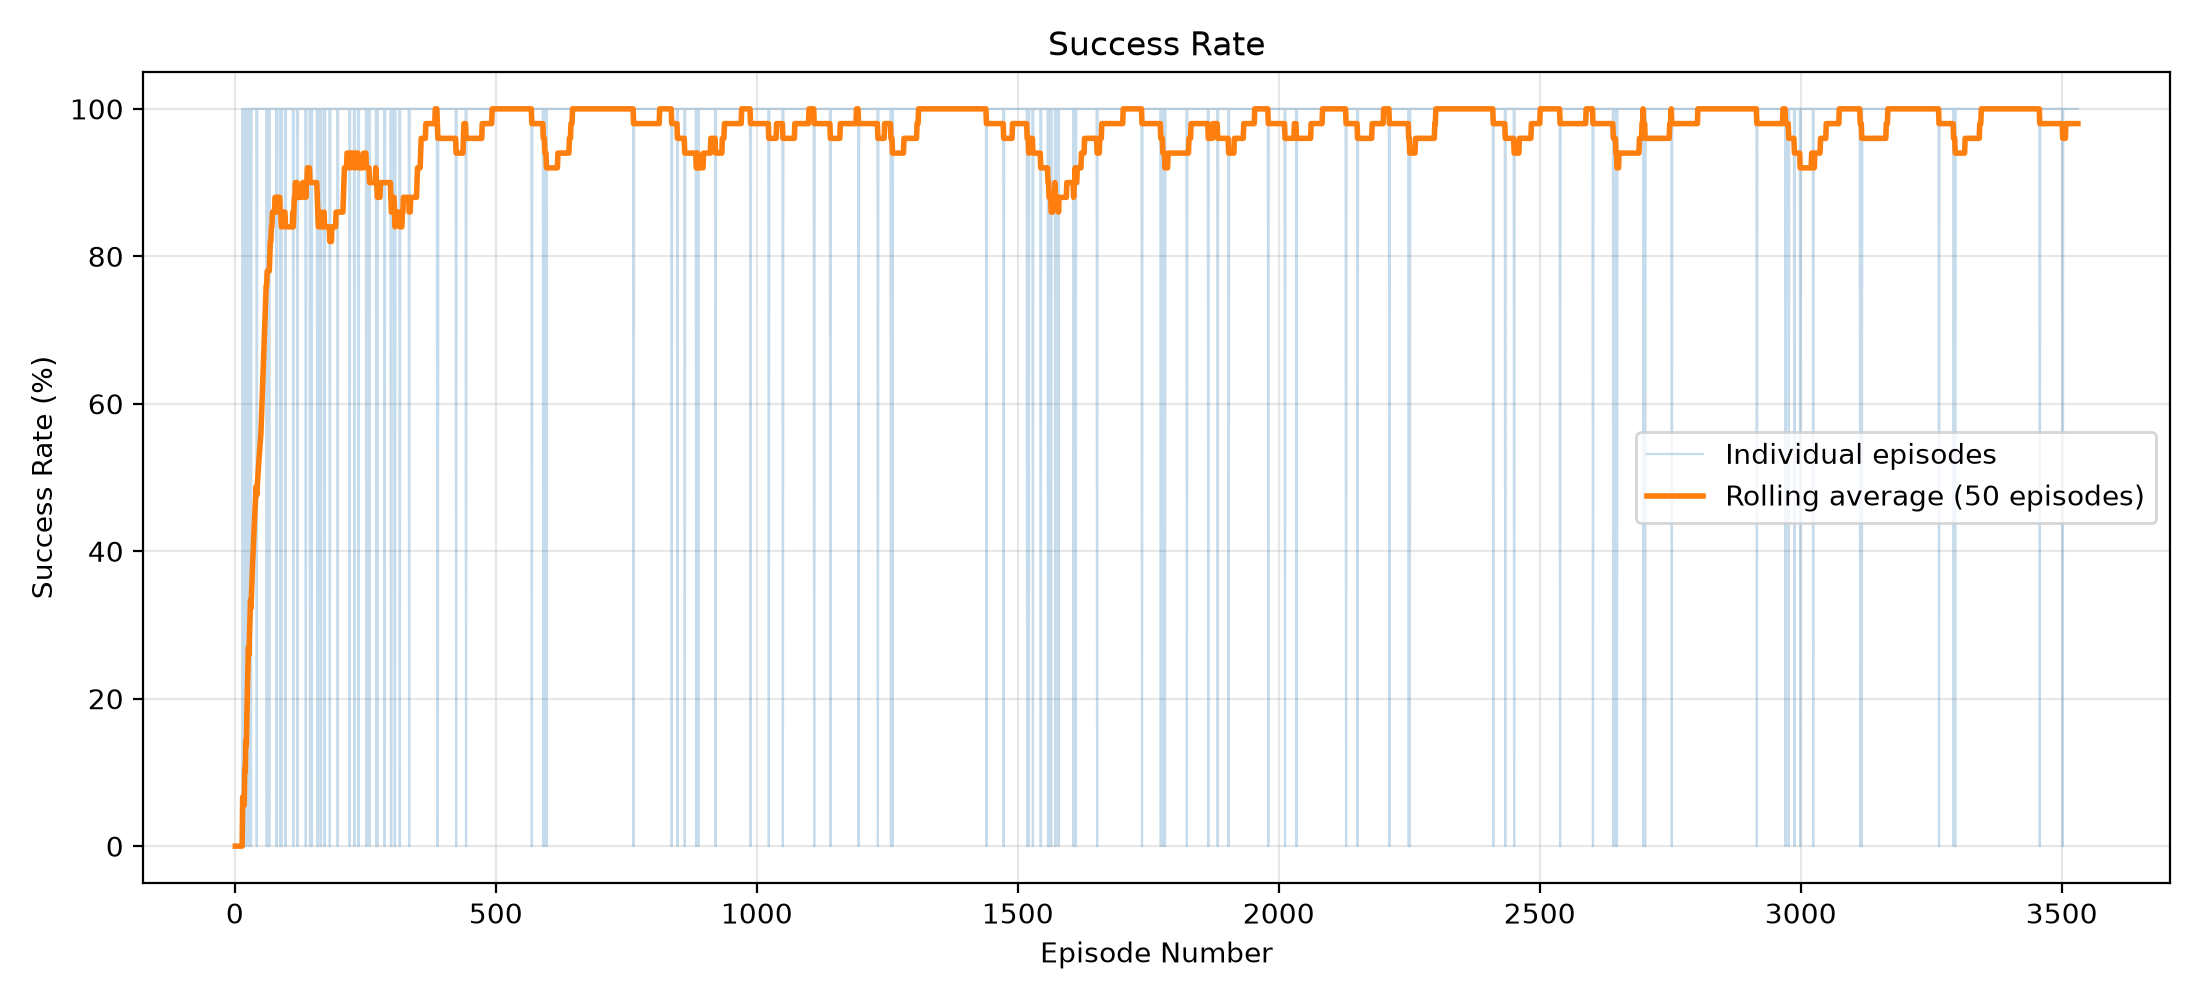
\includegraphics[width=\linewidth]{success_rate_sac_seed0.png}
    \caption{Success rate for one round of training with SAC}
    \label{fig:success_rate_sac_seed0}
\end{figure}

\begin{figure}[htbp]
    \centering
    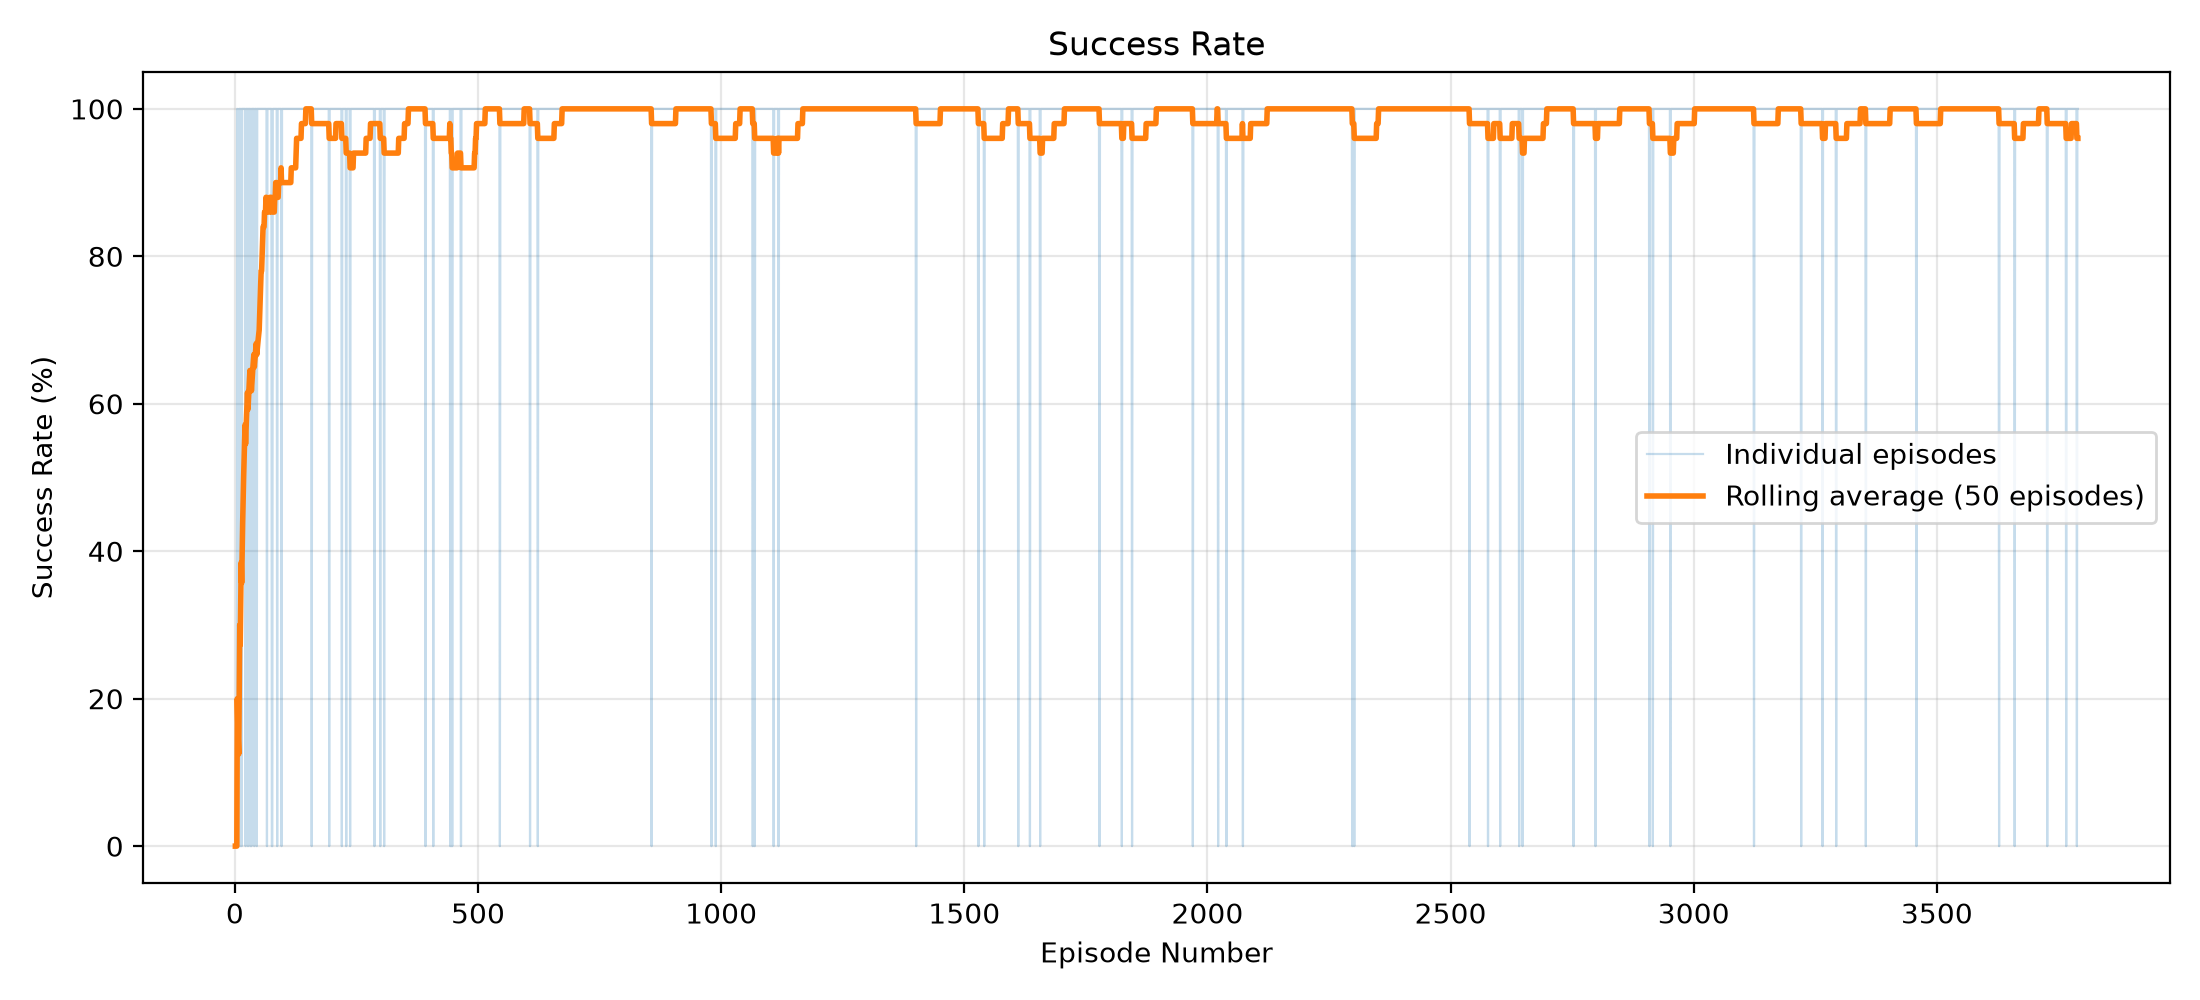
\includegraphics[width=\linewidth]{success_rate_td3_seed0.png}
    \caption{Success rate for one round of training with TD3}
    \label{fig:success_rate_td3_seed0}
\end{figure}

\begin{figure}[htbp]
    \centering
    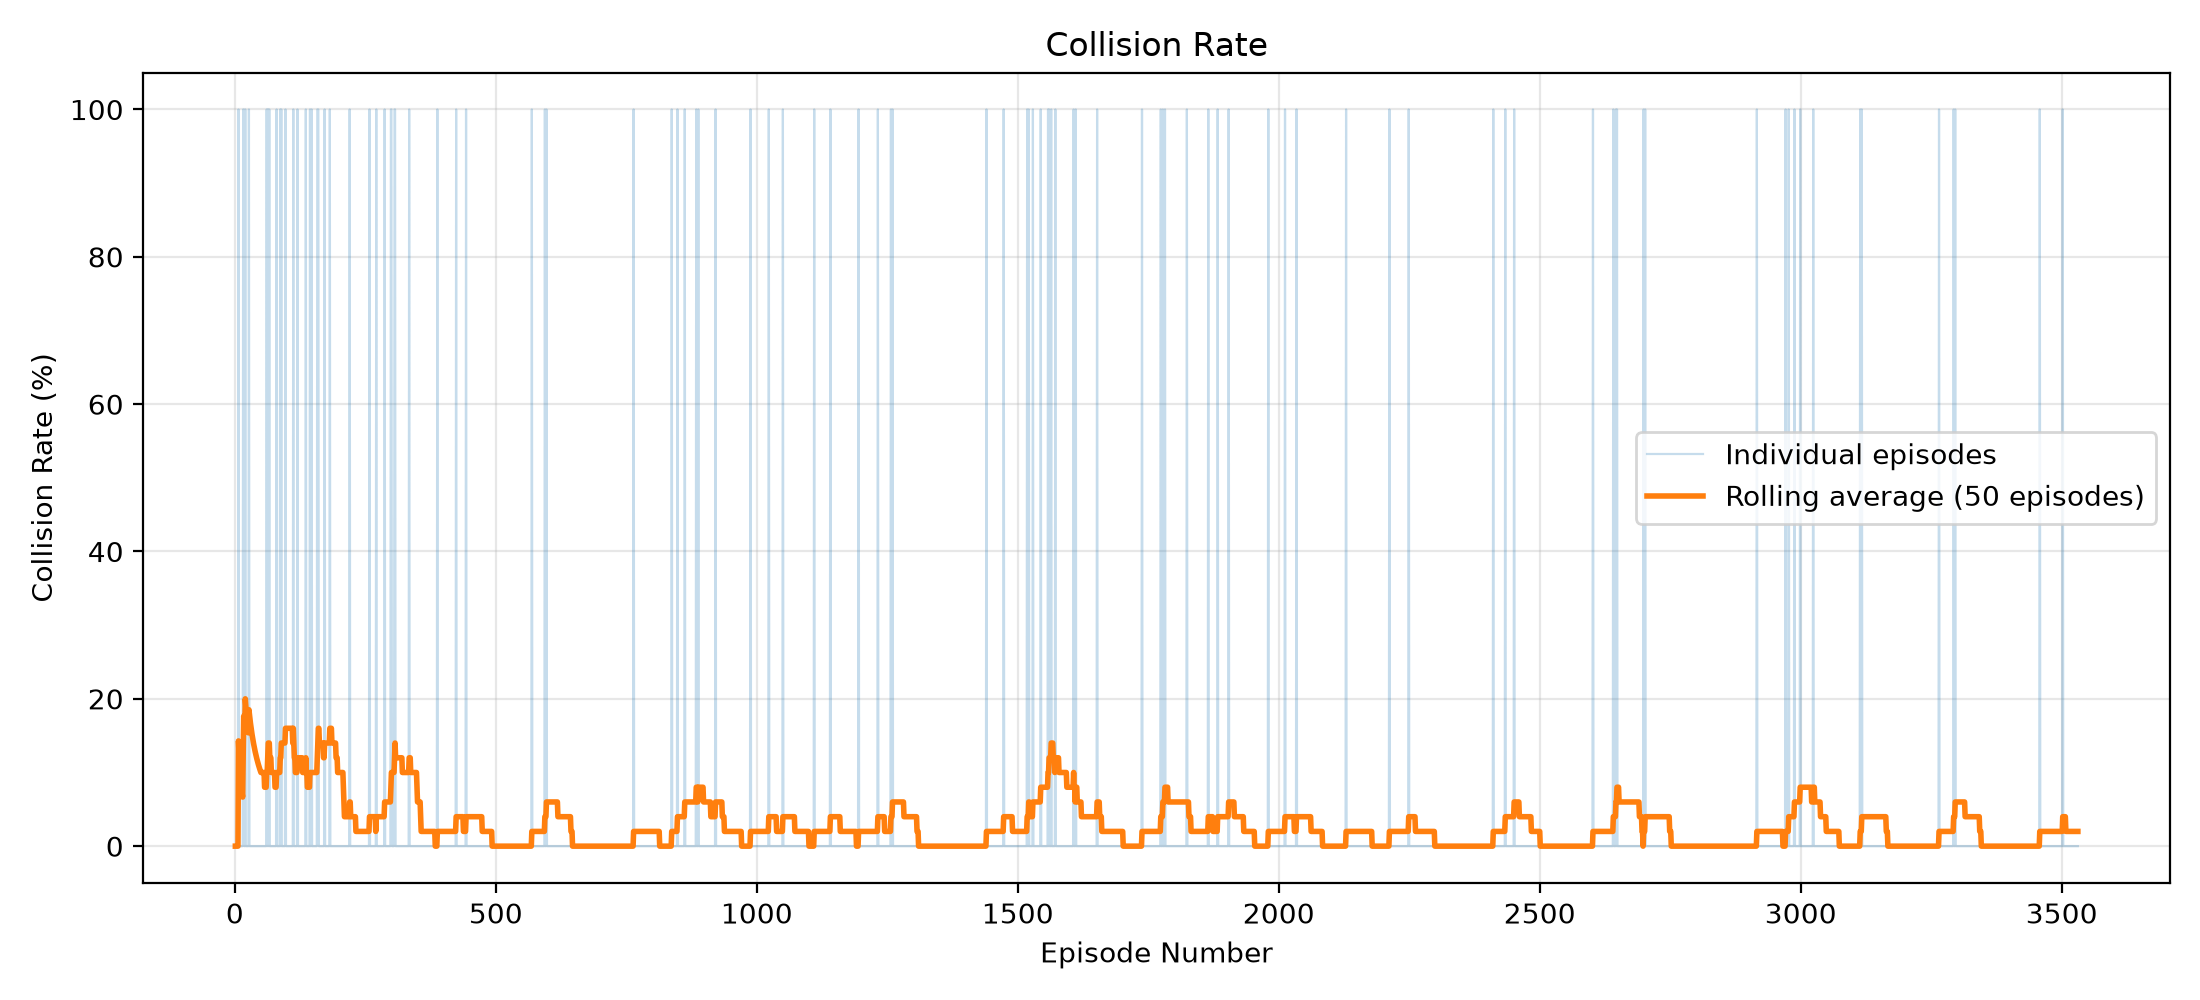
\includegraphics[width=\linewidth]{collision_rate_sac_seed0.png}
    \caption{Collision rate for one round of training with SAC}
    \label{fig:collision_rate_sac_seed0}
\end{figure}

\begin{figure}[htbp]
    \centering
    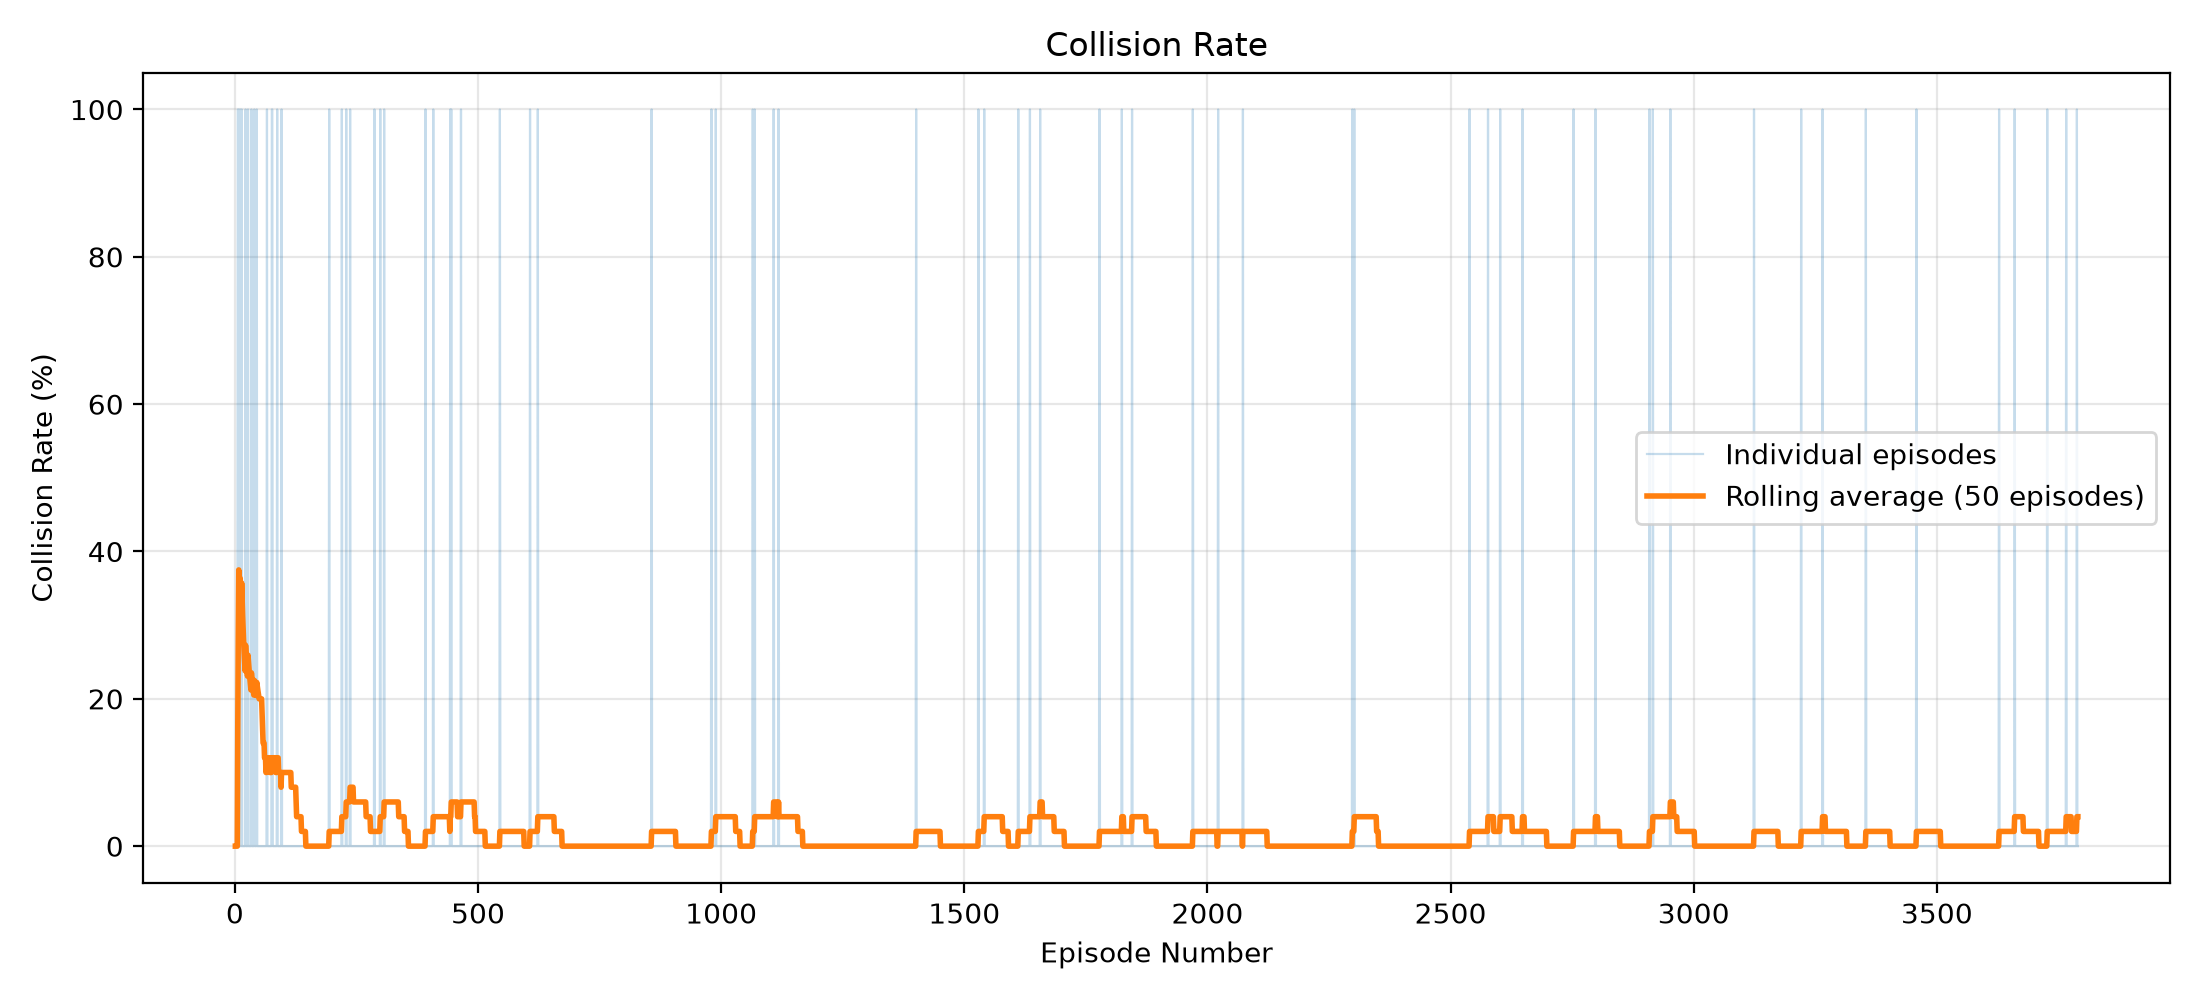
\includegraphics[width=\linewidth]{collision_rate_td3_seed0.png}
    \caption{Collision rate for one round of training with TD3}
    \label{fig:collision_rate_td3_seed0}
\end{figure}


\section{Tasks and Timeline}
Of the following tasks that we outlined in our initial paper, we have completed the first four of them. The remainder of our work this semester will be spent working on the sim-to-real pipeline to get a working implementation on the TurtleBot3.

\begin{enumerate}
    \item Understand the TurtleBot3 and ROS for physics-based simulations and real-world experiments.

    \item Understand basics of reinforcement learning, and more specifically, how it can be used for mobile robot navigation in an unknown environment.

    \item Develop the RL environment and reward function for SAC and TD3 algorithms, then complete training in simulated environments. 

    \item Implement the three methods (SAC, TD3, DWA) in a simulated environment to evaluate differences.

    \item Experiment with these algorithms in the real-world by testing them on the TurtleBot3.
\end{enumerate}

Our timeline for the rest of the semester:
\begin{itemize}
    \item November 23 - December 16

        \begin{itemize}
            \item Complete task 5.

            \item Write the final paper.

            \item Prepare for and give final presentation in class.
        \end{itemize}
    
\end{itemize}

\section{Risk Management}

Because we will be working with a physical robot, it is important to prioritize our safety and the safety of those around of us. In addition, because we will be using the TurtleBot3 for navigation in an obstacle-filled environment, we will need to find a suitable environment and obstacles that are robust to handle potential collisions with the TurtleBot3.

If we have questions or concerns, we will contact Travis Henderson, who manages the robots for MnRI.

Our project will start in a simulated environment and then transition into a real-world scenario, so we will also need to consider this sim-to-real gap and the problems that may arise, such as software and hardware compatibility on the TurtleBot3 compared with what we have running in our simulated environment.

Machine learning algorithms come with their own challenges that need to be overcome throughout the process of training and testing.
Some potential risks include RL training instability, failure to converge on a policy, excessive training time or computational costs, and overfitting of SAC or TD3 in the training environment.
Many of the risks faced during training can be mitigated through iterative reward-function refinement and hyperparameter tuning.
Other techniques to prevent overfitting and failure to converge would be to gradually increase the complexity and randomization of the training environments, while preserving unseen environments for testing.
Additionally, risks in excessive training time and computational costs could be mitigated either through the use of University-provided computational resources or by reducing the size of the observation space and down-sampling the LiDAR data. 



\bibliographystyle{IEEEtran}
\bibliography{citations}

\end{document}
